%*******************************************************************************
%*********************************** Chapter XXXXXXXX *****************************
%*******************************************************************************

\chapter{The 35 ton data sample}  %Title of chapter

\graphicspath{{35tonData/Figs/PDF/}{35tonData/Figs/Raster/}{35tonData/Figs/Vector/}}

The data taking period for the 35 ton prototype was from November 2015 until March 2016. This included an extensive commissioning period before the detector was filled with LAr and the electric field was turned on. During this time many of the features of the data discussed below were first noticed and attempts to rectify these were pursued. A long commissioning period was also required because many of the DAQ sub-systems were still under active development in November when the detector was sealed and filling began.\\

Over the whole run a total of 22 days worth of data was collected with the electric field set at 250 V cm$^{-1}$, the breakdown of these periods is shown in Figure~\ref{fig:DataCollected}. It is clear that the analysable data is interspersed with data where the electric field was not turned on, this is both due to extenuating circumstances such as a site wide power outage in early March and a dedicated two week noise hunting exercise in February. The physics data taking period ended at 3am on 19th March 2016 when a filtration pump broke causing an unrecoverable loss of purity as air was pumped into the detector. Following this studies to understand the electronics noise and test the high voltage systems continued but it was deemed impossible to acquire any more physics data. During this time the electric field was raised to the nominal value of 500  V cm$^{-1}$, and some of the causes of the higher than expected noise levels were discerned. This is explained further in \ref{All the noise}. 

\begin{figure}[htbp!]
  \centering
  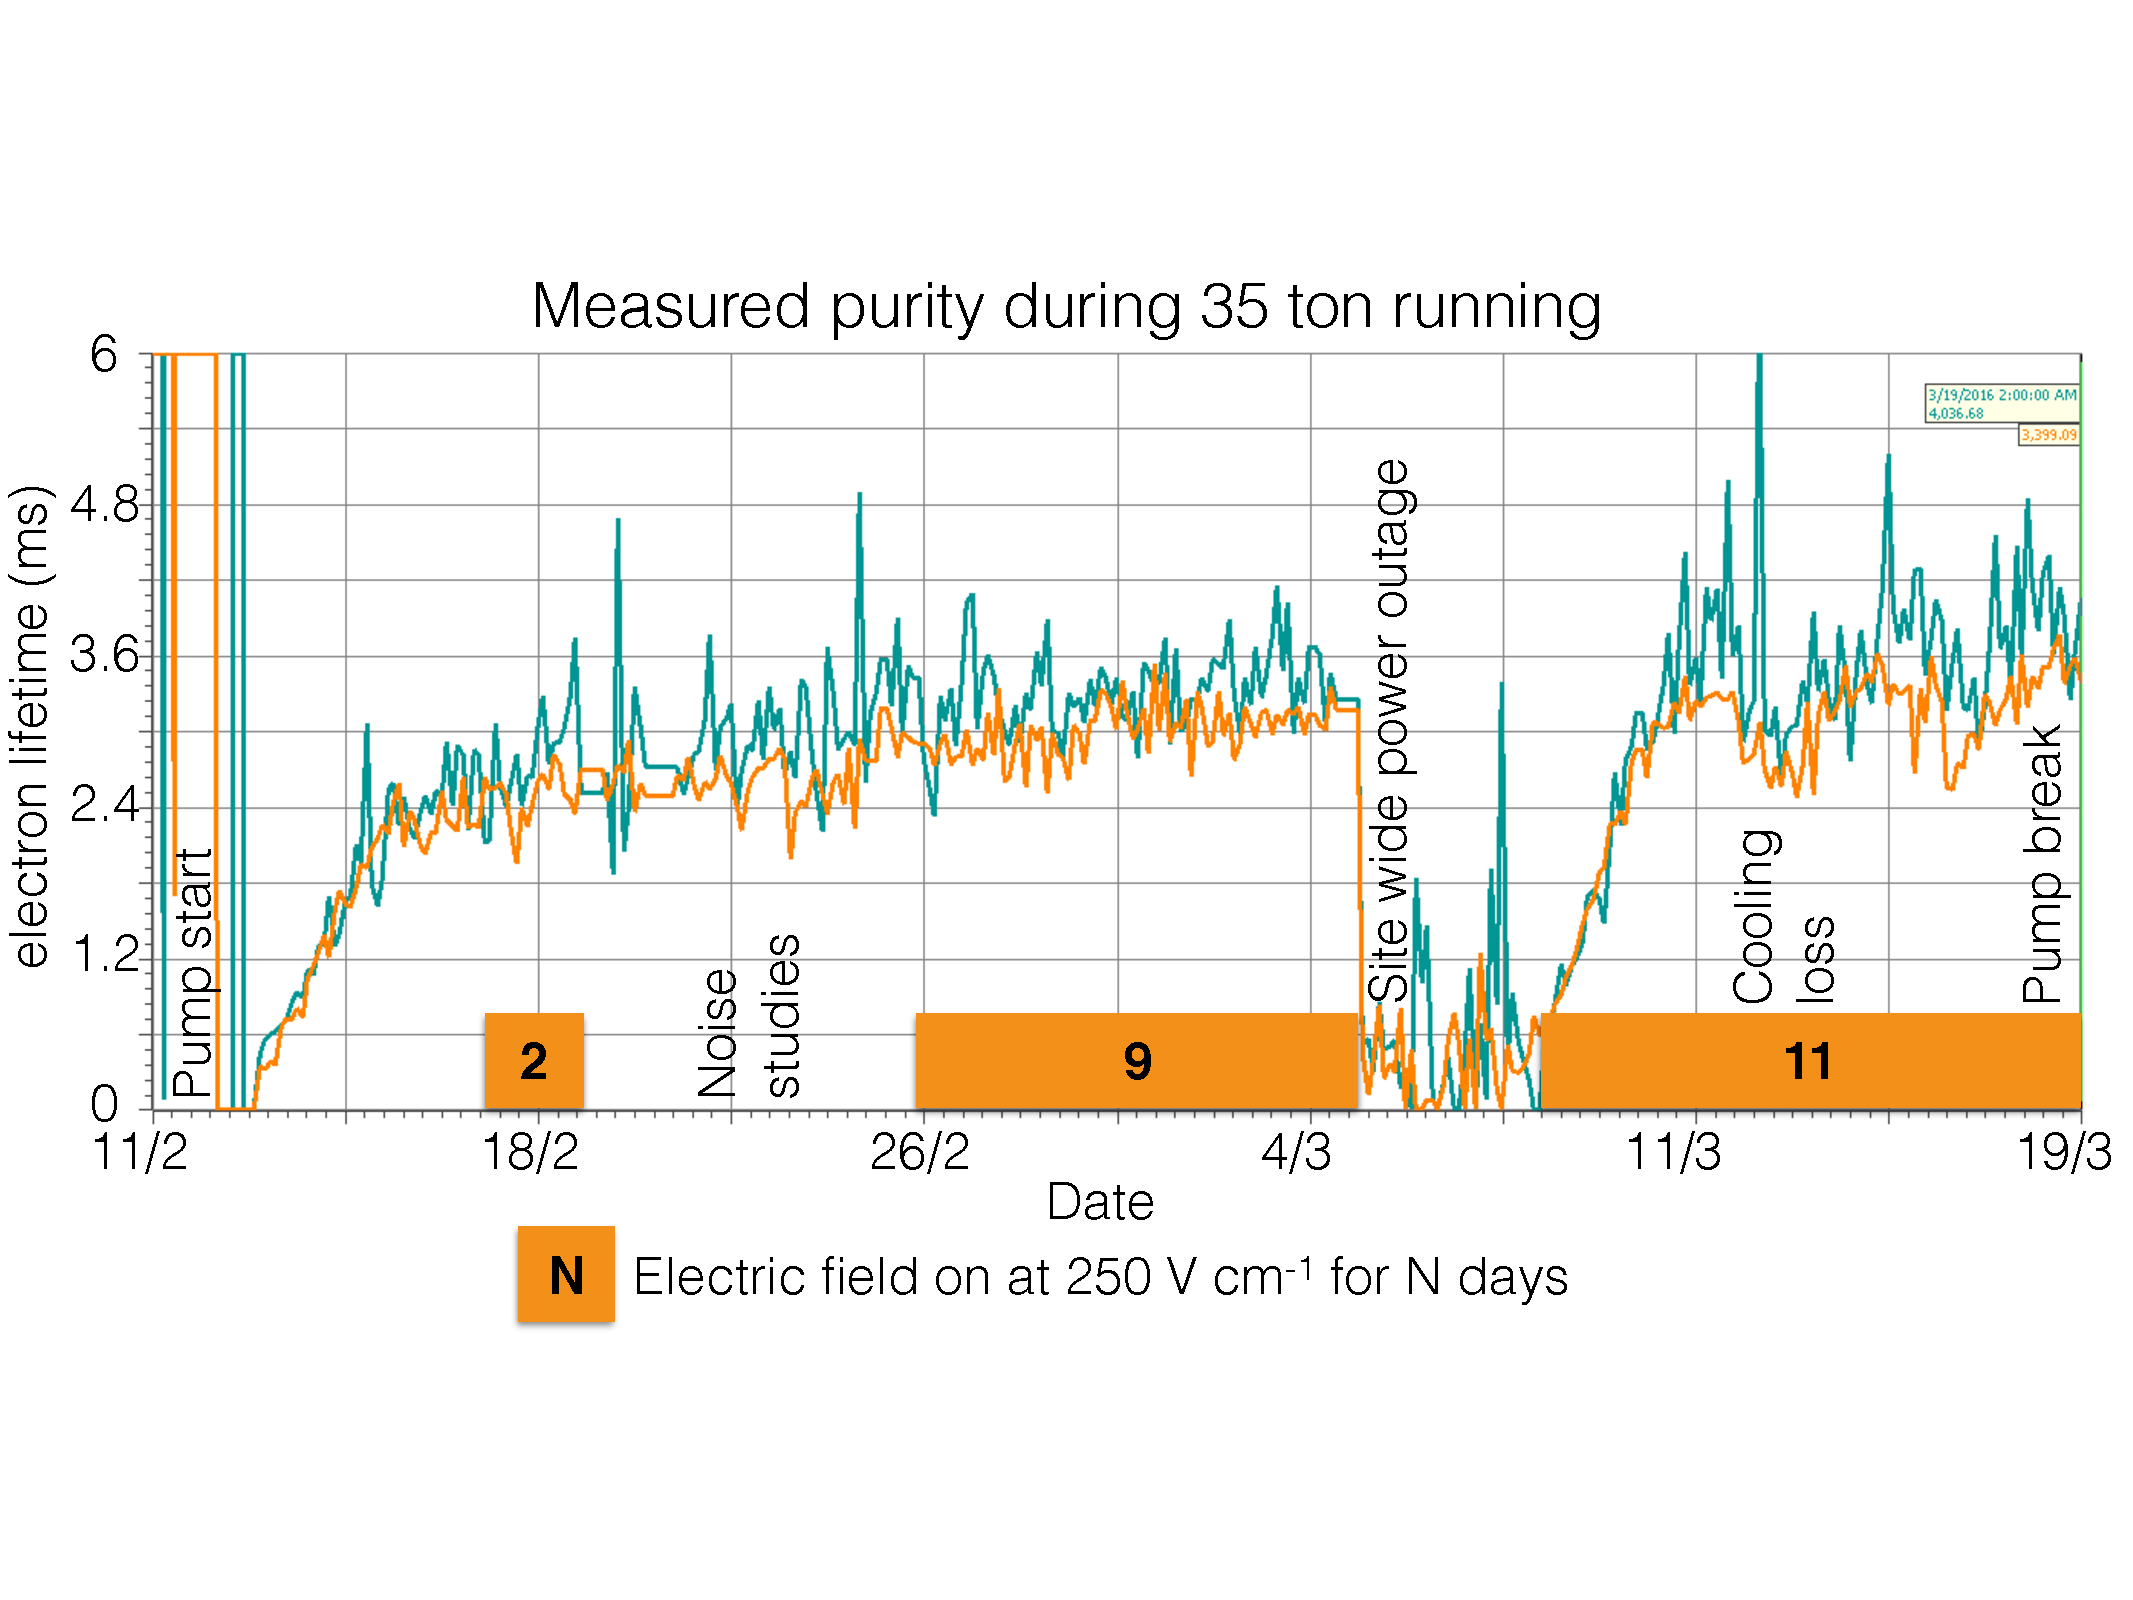
\includegraphics[width=1.0\textwidth]{DataCollected}
  \caption[DataCollected]{Timeline showing the data collected during the 35 ton Phase II run once the purification pumps were turned on.}
  \label{fig:DataCollected}  
\end{figure}


%********************************** %First Section  **************************************
\section{Organisation of the data structure} \label{Organisation of the data structure} %Section - X.1
As previously noted the 35 ton consisted of three detector sub-systems: RCEs collecting TPC data, SSPs collecting photon detector data, and CRCs collecting cosmic muon coincidences. The DAQ combined these three data streams into synchronous events in time saved as LArSoft objects called artdaq::Fragments. These data objects would later have to converted to the offline data products which the reconstruction tools developed on simulation used, this is discussed in \ref{Reformatting the data to the offline structure}. This section describes the structure of the data objects in the raw form.\\

During operations the DAQ was configured to maximise throughput and physics potential. This meant recording different lengths of times for each of the three sub-systems as the data volumes were significantly different. The maximum speed at which data could be written to disk was approximately 60 MB s$^{-1}$, this was roughly equal to the size of each triggered event when the entire detector was read-out in the configuration discussed below and so the 35 ton recorded events at roughly 1 Hz.\\

With an electric field of 250 V cm$^{-1}$ and a drift of 2.25 m, the drift time for electrons at the long drift CPA was roughly 2.6 ms or 5200 ticks (where 1 tick is 500 ns). It was decided that in order for a track causing a counter co-incidence to be separated from other tracks it was necessary to have one drift window both before and after the drift window around the co-incidence, meaning that data was recorded for 7.5 ms or 15,000 ticks around each co-incidence. The rate at which events were recorded could have been increased if zero-suppression had been used as data from the TPC was the dominant data being written out, however the elevated noise level meant that this was not feasible and so all ADC samples were recorded for all triggered events. The next most significant data volume was due to the SSPs which recorded data for XXXX $\mu$s around the trigger as this allows for the prompt light from the through-going particle to be collected. A larger time sample was not recorded to limit the data volume. The CRCs produced the least volume of data and so were able to be read out constantly, though the co-incidence triggers were only produced when a trigger was issued. The system used to collect the CRC data was also responsible for generating the triggers and so this meant that the production of triggers could be suppressed by only producing a trigger on the N$^{th}$ co-incidence. Without this feature the event rate would have been significantly higher, as the flux from muons triggering the vertical counters would have been over 60 Hz, before considering the horizontal co-incidences. \\

The time synchronous events produced by the DAQ did not however correspond to the physics events, this is because the DAQ was originally designed to produce a continuous data stream. This meant that the DAQ was configured to pad events with headers when there was a sub-system provided no physics information. Removing these padded header objects was a further remit of the online to offline converter discussed in \ref{Reformatting the data to the offline structure}. The length of the DAQ events was configurable and was chosen to be 10 ms (20,000 ticks) in order to best attempt to fully contain physics events and reduce the need for the online to offline converter to stitch DAQ events together. The padding of DAQ events with headers between physics events introduced some peculiarities in the data recorded such as DAQ events containing two parts of non-continuous data as shown in Figure~\ref{fig:DataStructure} where the second DAQ event has no information for time between the end of physics event 2 and the start of physics event 3.\\

\begin{figure}[htbp!]
  \centering
  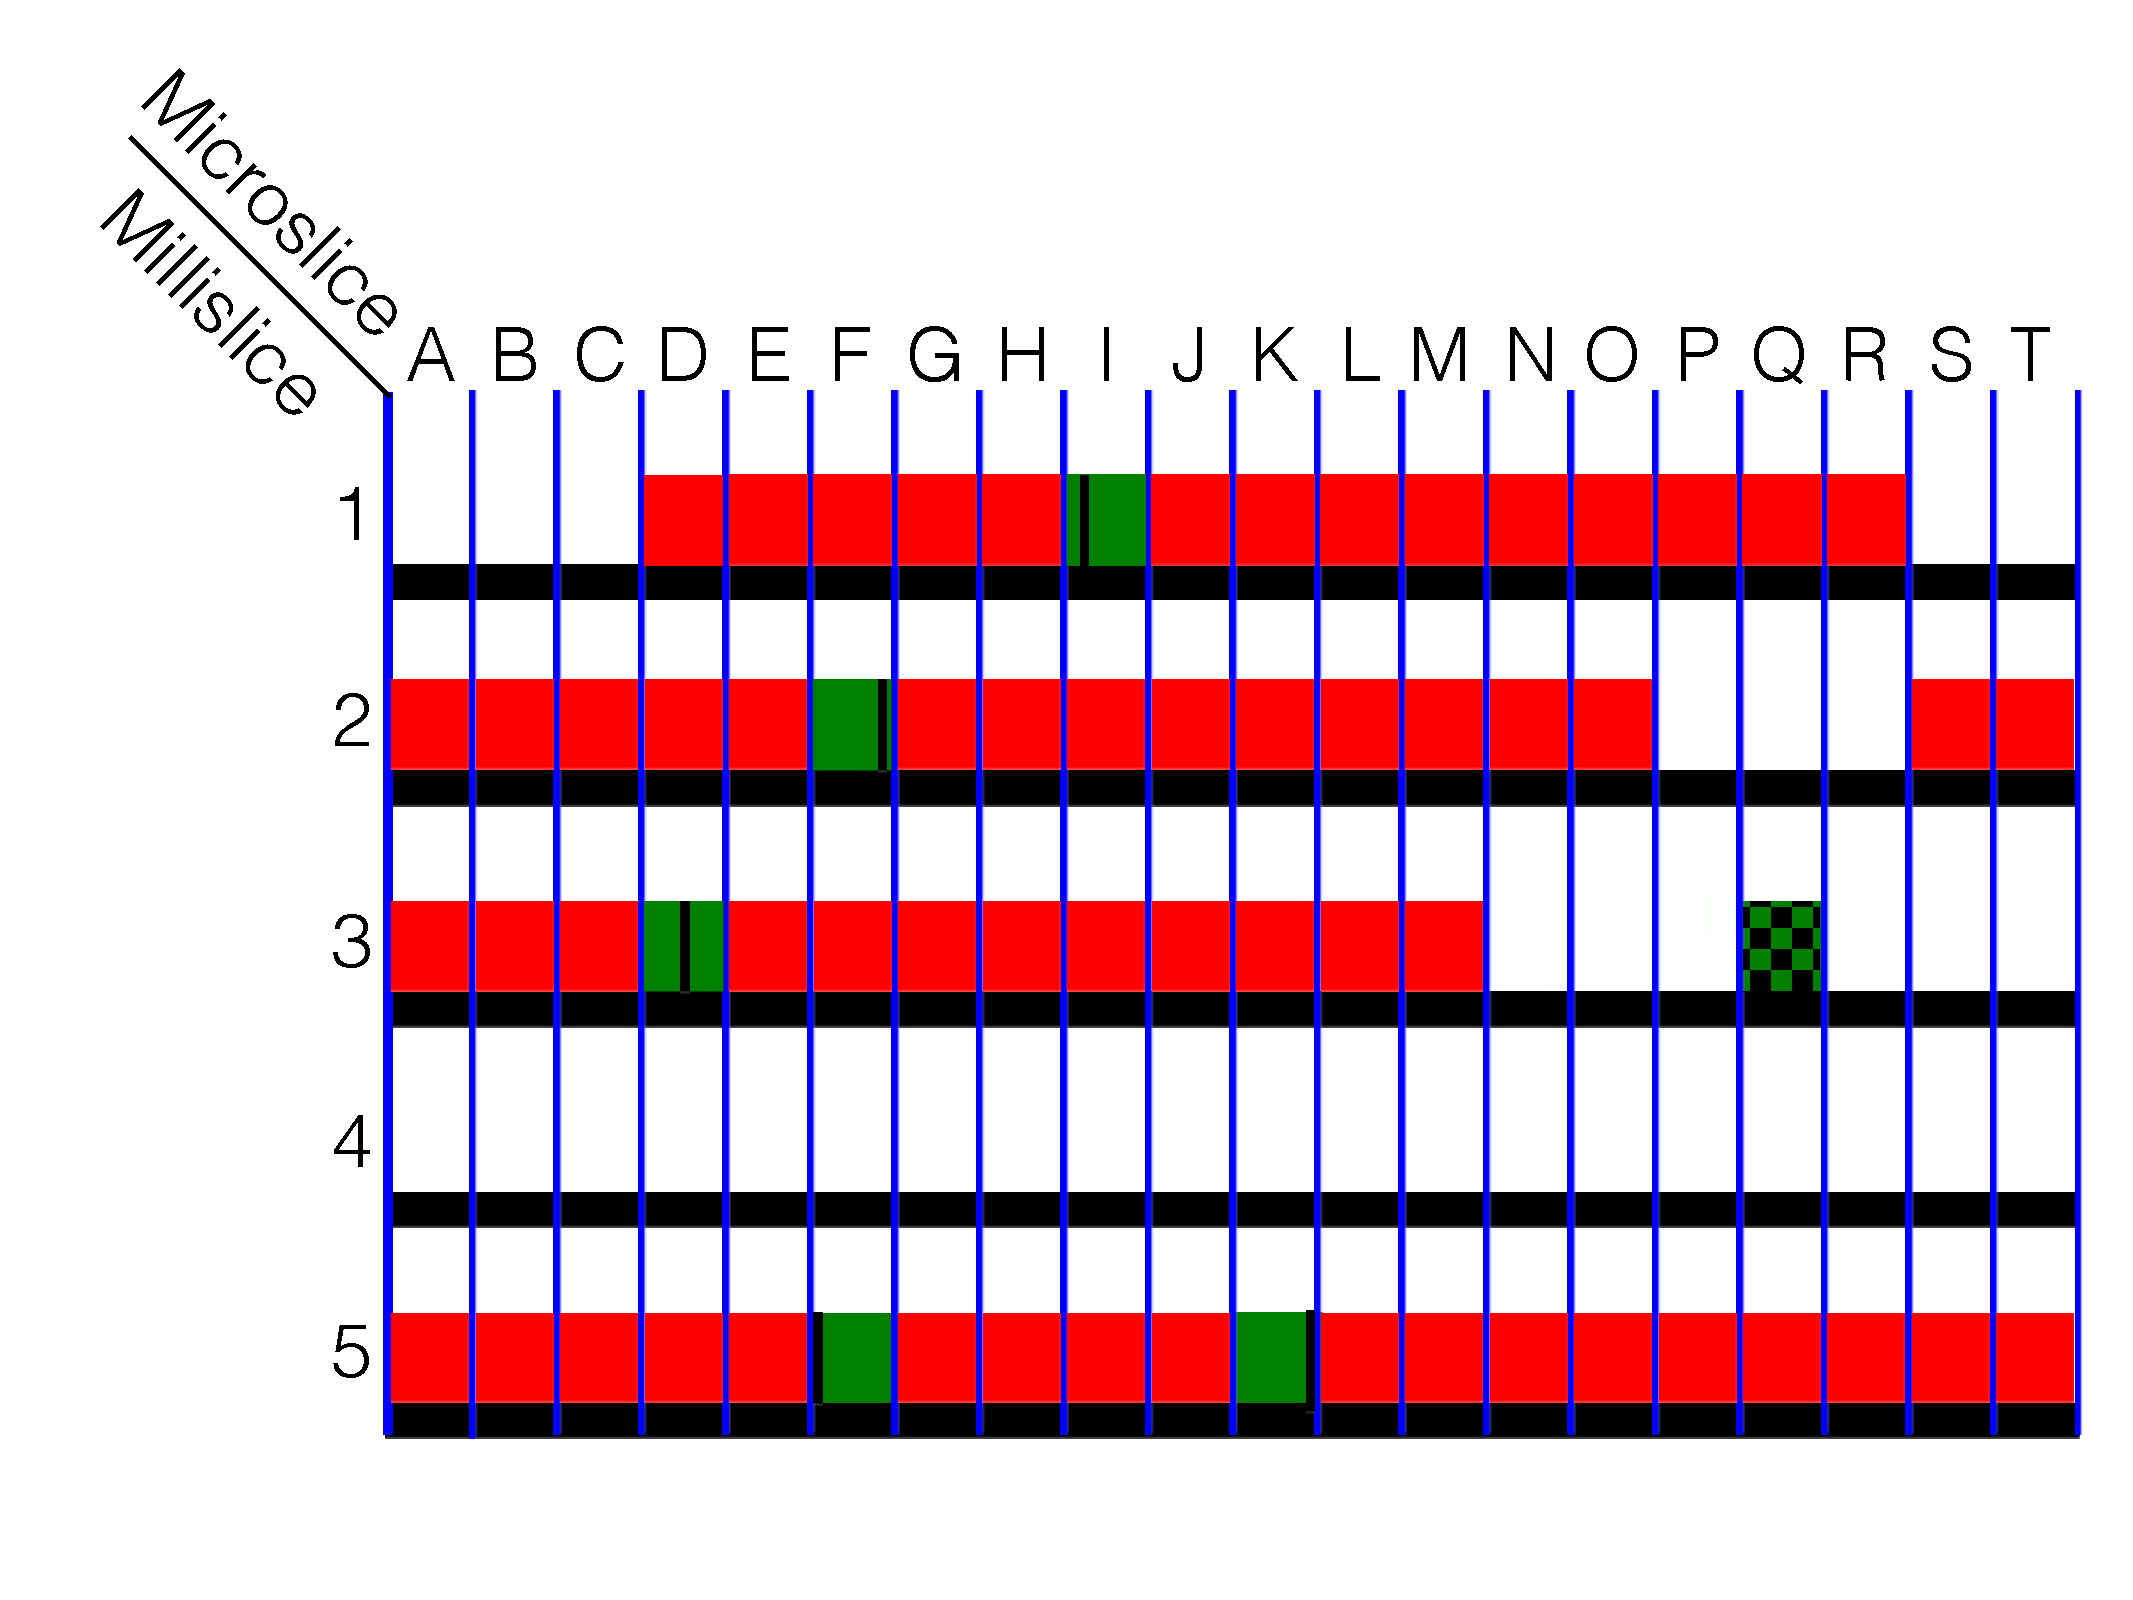
\includegraphics[width=0.75\textwidth]{DataStructure}
  \caption[DataStructure]{A diagram of possible microslice structures for the TPC data recorded by the 35 ton. Each row represents a single DAQ event. The vertical blue lines delineate each microslice (0.5 ms, 1,000 ticks). Solid red boxes represent micro slices with TPC data in them. Green boxes represent triggers which were used with the black lines showing the time at which the trigger occurred, and dashed green and black boxes represent triggers which were ignored.}
  \label{fig:DataStructure}
\end{figure}

As the run mode required accessing buffered data it had to be discretised inside the components before being sent to the event builders in the DAQ. In the discussion of how this worked focus will be given on the RCE data where some new terms need to be introduced. Data is collected for every tick on each RCE, where each RCE controls 128 channels. This is called a nanoslice. A microslice is then made by combining N nanoslices such that it contains 0.5 ms (1,000 ticks) of data across all channels. Microslices are then combined to make millislices, where a millislice is synonymous with the DAQ events discussed earlier meaning that 20 microslices are combined to make a millislice. A lack of recorded data means that microslices consist of headers in the place of nanoslices. \\

During normal data taking the last N microslices are buffered in the RCEs so that if a trigger is issued the previous millislices can be accessed before they are deleted. As the data is buffered in the form of microslices previous millislices may only be accessed in whole. This means that a whole number of millislices must be loaded before the trigger so when a trigger is issued part way through a millislice the previous X millislices are sent to the event builders. As a result during there are always a minimum number of ticks both before (5,000 ticks) and after the trigger (9,000 ticks) but the exact numbers can change by up to 1,000 ticks for a given event depending on where in a millislice the trigger comes. This is shown in Figure~\ref{fig:DataStructure} where the black lines representing triggers are seen to occur at different points within the microslices, for example physics event 1 will have more data after the trigger than physics event 2 as the trigger occurs earlier in the triggered microslice. \\

The information in this section has been summarised in FigureXXX and FigureXXX below.

%********************************** %Second Section  *************************************
\section{Reformatting the data to the offline structure} \label{Reformatting the data to the offline structure} %Section - X.2
Conversion of the raw data in the form of artdaq::Fragments to LArSoft objects such as raw::RawDigits (TPC), raw::ExternalTrigger (CRC) and recob::OpDetWaveforms (SSP) required a suite of unpacking services to be written the specifics of which are not discussed here. These all required a common interface through which to access the data, check that the timing of each component was consistent and then produce a final LArSoft file for downstream use. This programme had the added role of producing complete physics events, meaning that it had to be able to combine multiple millislices and extract only the time sample containing the continuous physics events. \\

The basic format that the data reformatter followed was that following the unpacking of each of the sub-systems the TPC ticks would be looped through to see if a user defined set of conditions could be satisfied. These conditions were usually whether an East-West or North-South counter-coincidence occurred at that time, or if the current millislice contained TPC data whilst the previous one did not. The latter was the default configuration as this gave the option of preserving all of the data gathered. Other conditions were available though rarely used such as if a threshold of recob::OpDetWaveforms was exceeded, corresponding to a large flash of light. Once a set of conditions is satisfied a user defined number of pre-condition ticks are gathered, clearly this is set to zero in the case of the previous millislice containing no TPC data as there is no previous data to load which would not have a gap in time, see Figure~\ref{fig:DataStructure}. In the case of using a counter co-incidence to make an event a value of 300 pre-condition ticks is normally used. Once the pre-conditions ticks are gathered a further N post-condition ticks are gathered, where N is defined by the user. Usually 15,000 ticks are gathered when the previous millislice is empty and 5,200 ticks are gathered when there is a co-incidence. Once the required volume of TPC is collected, data from the other components is added to the event if its timestamp is within the timestamps of the first and last ticks in the event. All timestamps were then corrected such that the event began at T=0 as the reconstruction assumes this, the start time of the event was then stored in the event record so that it could accessed downstream. \\

fsdfsd

%********************************** % Third Section  *************************************
\section{Observations on data quality}  %Section - X.3

%********************************** % Fourth Section  *************************************
\section{Noise suppression, mitigation and warm tests}  \label{All the noise}%Section - X.4

%********************************** % Fifth Section  *************************************
\section{Performance of reconstruction algorithms}  %Section - X.5

%********************************** % Sixth Section  *************************************
\section{???Measuring interaction times using electron diffusion???}  %Section - X.6 

